\documentclass[a4paper,12pt,landscape,twocolumn]{article}

\usepackage{préambule}
\usetikzlibrary{calc,arrows.meta}
\usepackage{clipboard}

\geometry{left=1cm}
\setlength{\columnsep}{0.8cm}

\newcommand{\myarrow}{{Latex[length=1mm, width=1.5mm]}-{Latex[length=1mm, width=1.5mm]}}

\newcommand{\correction}[1]{{\color{red}#1}}

\TitreDEvaluation{Évaluation calcul littéral 2}
\author{}
\date{6 mai}

\begin{document}

\renewcommand{\arraystretch}{1.4}

\Copy{Contenu}{
	\maketitle

	\begin{exercice}\

		\begin{center}
			\begin{tikzpicture}[scale=0.95]
				\coordinate (A) at (0,0);
				\coordinate (B) at (3,0);
				\coordinate (C) at (6,0);
				\coordinate (D) at (9,0);
				\draw[|-|] (A) -- node {/} (B);
				\draw[|-|] (B) -- node {/} (C);
				\draw[|-|] (C) -- node {/} (D);

				\foreach \p in {A,B,C,D} {
						\node[below] at ($(\p) - (0,0.15)$) {\p};
					}

				\draw[\myarrow] ($(A) - (0,0.84)$) -- node[below] {$x$} ($(B) - (0,0.84)$);
			\end{tikzpicture}
		\end{center}

		On appelle $x$ la distance AB.

		Écrire une expression représentant la distance AD : \correction{$3x$}

		\vspace{0.9em}

		\begin{center}
			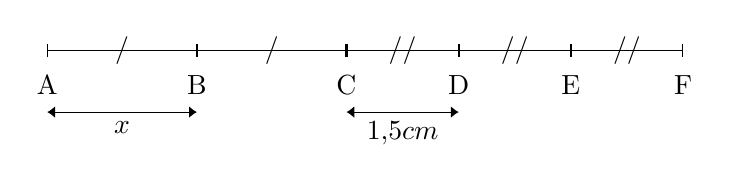
\begin{tikzpicture}[scale=0.95]
				\coordinate (A) at (0,0);
				\coordinate (B) at (2,0);
				\coordinate (C) at (4,0);
				\coordinate (D) at (5.5,0);
				\coordinate (E) at (7,0);
				\coordinate (F) at (8.5,0);
				\draw[|-|] (A) -- node {/} (B);
				\draw[|-|] (B) -- node {/} (C);
				\draw[|-|] (C) -- node {//} (D);
				\draw[|-|] (D) -- node {//} (E);
				\draw[|-|] (E) -- node {//} (F);

				\foreach \p in {A,B,C,D,E,F} {
						\node[below] at ($(\p) - (0,0.2)$) {\p};
					}

				\draw[\myarrow] ($(A) - (0,0.82)$) -- node[below] {$x$} ($(B) - (0,0.82)$);
				\draw[\myarrow] ($(C) - (0,0.82)$) -- node[below] {$1{,}5 cm$} ($(D) - (0,0.82)$);
			\end{tikzpicture}
		\end{center}

		On appelle $x$ la distance AB. De plus, on sait que la distance CD est $1{,}5$cm.

		Écrire une expression représentant la distance AF : \correction{$2x + 4{,}5cm$}
	\end{exercice}

	\begin{exercice}\

		Calculer la valeur de l'expression $6 × x$ pour : \vspace{0.5em}

		\begin{tabular}{lll}
			a. & $x = 4$ : & \correction{$24$} \\
			b. & $x = 8$ : & \correction{$48$} \\
		\end{tabular}
	\end{exercice}

	\begin{exercice}\

		Calculer la valeur de l'expression $3 × x + 6 - 2 × y$ pour : \vspace{0.5em}

		\begin{tabular}{lll}
			a. & $x = 6$ et $y = 5$ :  & \correction{$14$} \\
			b. & $x = 8$ et $y = 15$ : & \correction{$0$}  \\
		\end{tabular}
	\end{exercice}

	\begin{exercice}\

		Simplifier les expressions suivantes : \vspace{0.5em}
		\begin{enumerate}[label=\alph*.]
			\setlength\itemsep{5pt}
			\item $2{,}5 × x = $ \correction{$2{,}5x$}
			\item $x + x + x + 2{,}5 - 1 = $ \correction{$3x + 1{,}5$}
			\item $7 × x + 2 × y  - 1 × x = $ \correction{$7x + 2y - x = 6x + 2y$}
		\end{enumerate}
	\end{exercice}
}

\newpage

\setcounter{exercice}{0}
\Paste{Contenu}

\end{document}